% ============================================================================
% Introduction
%
% Author Goals:
% - Orient the reader.
% - Explain why this research matters.
% - Introduce the research gap.
% - State the contribution.
% - Foreshadow the remainder of the paper.
% ============================================================================

\documentclass[11pt]{article}

\usepackage[a4paper,margin=2.5cm]{geometry}
\usepackage{graphicx}
\usepackage{booktabs}
\usepackage{longtable}
\usepackage{float}
\usepackage{amsmath}
\usepackage[hidelinks]{hyperref}

% Custom command to open links in a new tab
\newcommand{\hrefblank}[2]{%
  \href{#1}{\nolinkurl{#2}}%
}


\title{Transition Analysis Toolkit\\
A Reproducible Framework for Analysing Student Transition Pathways}

\author{Jason Stanley}

%\date{\today}
\date{
Version 0.9\\[0.5em]
Draft for Review\\[1em]
\today
}

\begin{document}

\maketitle

\setlength{\parskip}{0.4em}
\linespread{1.10}\selectfont

\begin{abstract}

Student transition into first-year university mathematics remains a significant challenge for higher education institutions, with differences in prior mathematical 
preparation strongly influencing subsequent academic success. This study investigates factors associated with successful transition into a first-stage undergraduate 
mathematics subject using the Transition Analysis Toolkit, a reproducible analytical framework that integrates statistical analysis, interpretable machine learning, 
independent verification, and automated publication generation. Decision tree and random forest models were developed and compared using a reproducible analytical 
workflow to evaluate predictive performance and the relative importance of educational predictors. Across all evaluated models, secondary mathematics preparation 
consistently emerged as the strongest predictor of academic success, followed by composite risk measures and preparatory mathematics. Beyond the empirical findings, 
the principal contribution of this research is the development of a reproducible workflow that links data preparation, statistical 
modelling, machine learning, independent verification, automated reporting, and manuscript generation within an integrated framework for educational research. 
The framework demonstrates how reproducible analytical workflows can support interpretable educational data analytics while ensuring consistency between analytical 
outputs and published results. It provides a reusable foundation for future investigations of student transition, progression, and academic success across 
educational contexts and supports evidence-informed institutional decision-making.



\vspace{1.75em}

\noindent\small\textbf{Keywords:}
student transition; university mathematics; mathematical preparedness;
interpretable machine learning; reproducible research

\end{abstract}

%\tableofcontents


\normalsize

\newpage

\newcommand{\SecondaryMathImportance}{0.276}
\newcommand{\CompositeRiskImportance}{0.238}
\newcommand{\PreparatoryMathImportance}{0.232}
\newcommand{\TopThreeImportance}{74.6}


\newcommand{\HighestROCAUC}{0.766}
\newcommand{\LowestROCAUC}{0.756}
\newcommand{\BestROCModel}{Decision Tree — With Risk}
\newcommand{\BestROCAUC}{0.766}
\newcommand{\TunedROCModelCount}{4}
\newcommand{\TunedROCModelCountWord}{four}


% 1. What educational problem motivates this research?
%
% 2. Why is this problem important?
%
% 3. What gap in current knowledge or practice does this study address?
%
% 4. What does this research contribute?
%
% 5. How is the remainder of the paper organised?

\section{Introduction}

The transition from secondary school to first-year university mathematics presents a well-documented challenge for many students entering science, engineering, and related 
disciplines\\ \cite{Clark2009understanding}. Differences in prior mathematical preparation, curriculum pathways, and academic readiness contribute to substantial variation 
in students' achievement and persistence during the first year of university study~\cite{Hourigan2007underpreparedness}. For universities, understanding these factors is 
important for informing curriculum design, identifying students who may benefit from targeted academic support, and developing evidence-based transition initiatives~\cite{Thomas2008}. 
This study investigates the factors associated with successful transition into first-year university mathematics with the aim of providing evidence to inform institutional 
decision-making and support student success.

Over the past two decades, considerable research has examined the factors associated with success in first-year university mathematics, including prior academic achievement, 
secondary school mathematics preparation, demographic characteristics, and measures of academic preparedness~\cite{Clark2009understanding,England2021transition}. More recently, 
advances in educational data analytics and machine learning have enabled increasingly sophisticated approaches to modelling student performance~\cite{Koedinger2013data,Heffernan2023}. While these 
approaches have improved predictive capability, there remains a need for analyses that not only identify influential predictors but also provide interpretable evidence of their relative importance 
in ways that are meaningful for educational decision-making. This study addresses that need through a transparent and reproducible analytical framework that combines predictive modelling with 
educational interpretation to investigate the factors associated with successful transition into first-year university mathematics.

This paper presents a reproducible framework for analysing student transition pathways into first-stage undergraduate mathematics through an integrated analytical workflow combining 
statistical analysis, interpretable machine learning, independent verification, and automated reporting. As a case study, the framework is applied to investigate factors 
associated with successful transition into a first-stage undergraduate mathematics subject using multiple tuned decision tree and random forest models. Rather than advocating 
a single predictive model, the study emphasises consistency of interpretation across modelling approaches and demonstrates how transparent, reproducible analytical workflows 
can support educational research. The principal contribution is therefore not a new predictive algorithm, but a reusable research framework that integrates data preparation, 
model development, independent verification, interpretation, and publication-ready reporting within a single reproducible pipeline.

\subsection{Research Questions}

\begin{enumerate}
\item Which factors are the strongest predictors of success in first-year university mathematics?
\item How consistent are predictor importance rankings across multiple machine learning models?
\item What educational insights emerge from interpreting the tuned models?
\end{enumerate}


% ============================================================================
% Methodology
%
% Purpose
% -------
% Explain HOW the research was conducted, not WHAT was discovered.
%
% Reader should understand:
%   • the overall research workflow
%   • why the analysis is reproducible
%   • the research dataset
%   • variables analysed
%   • statistical methods
%   • machine learning models
%   • independent R verification
%   • automated reporting pipeline
%
% Do NOT discuss:
%   • model performance
%   • feature importance
%   • educational interpretation
%   • conclusions
%
% Transition:
% This section prepares the reader to understand and trust the Results.
% ============================================================================


\section{Methodology} 

This study adopted a reproducible analytical workflow to investigate factors associated with successful transition into first-year university mathematics. 
The workflow was designed to ensure that each stage of the analysis, from data preparation through statistical modelling, independent verification, and report 
generation, could be reproduced from the original research dataset using an automated build process. This approach emphasises transparency, repeatability, and 
traceability, allowing both analytical results and publication outputs to be generated consistently from the same underlying evidence.

% --------------------------------------------------------------------------
% Research workflow
%
% Explain the overall analytical process before introducing individual
% components such as the dataset and modelling methods.
%
% This subsection establishes reproducibility as the guiding principle.
% --------------------------------------------------------------------------
\subsection{Research Workflow}

This study followed a reproducible analytical workflow consisting of data preparation, statistical analysis, machine learning model development, independent 
verification using R, and automated generation of publication-ready tables, figures, and manuscript components. Each stage formed part of an integrated build 
process, ensuring that analytical outputs could be reproduced directly from the underlying research dataset.

Figure~\ref{fig:workflow} summarises the reproducible analytical workflow used in this study, from preparation of the approved research dataset through 
statistical analysis, machine learning, independent verification, and automated publication outputs.

\begin{figure}[htbp]
\centering

\fbox{
\begin{minipage}{0.92\textwidth}
\centering

\textbf{Institutional Source Data}

\vspace{0.15cm}
$\downarrow$

\vspace{0.15cm}
\textbf{Data Preparation}

\vspace{0.15cm}
$\downarrow$

\vspace{0.15cm}
\textbf{Research Dataset}

\vspace{0.15cm}
$\downarrow$

\vspace{0.15cm}
\begin{tabular}{c@{\hspace{1.5cm}}c}
\fbox{\parbox{0.30\textwidth}{\centering
\textbf{Statistical Analysis}
}}
&
\fbox{\parbox{0.30\textwidth}{\centering
\textbf{Machine Learning Analysis}
}}
\end{tabular}

\vspace{0.15cm}

\[
\searrow \hspace{2.8cm} \swarrow
\]

\vspace{0.15cm}
$\downarrow$

\vspace{0.15cm}
\textbf{Independent Verification (R)}

\vspace{0.15cm}
$\downarrow$

\vspace{0.15cm}
\textbf{Tables • Figures • Generated LaTeX Values}

\vspace{0.15cm}
$\downarrow$

\vspace{0.15cm}
\textbf{Publication-ready Paper}

\end{minipage}
}

\caption{Reproducible analytical workflow implemented by the Transition Analysis Toolkit. Institutional data are transformed into an approved 
de-identified research dataset before parallel statistical and machine learning analyses are independently verified in R. Automated generation 
of tables, figures, LaTeX variables, and manuscript content ensures consistency between the analytical outputs and the final publication.}

\label{fig:workflow}

\end{figure}



% --------------------------------------------------------------------------
% Research Dataset
%
% Purpose
% -------
% Describe the research data used in this study.
%
% Reader should understand:
%   • where the data came from
%   • who is represented
%   • ethical considerations
%   • why the dataset is appropriate
%
% Do NOT discuss:
%   • model results
%   • predictor importance
%   • interpretation
%
% Transition:
% The next subsection describes the variables derived from this dataset.
% --------------------------------------------------------------------------
\subsection{Research Dataset} 

The study used de-identified institutional data from students enrolled in a first-stage undergraduate mathematics subject offered during the Autumn 2026 teaching session. The dataset was prepared specifically for research purposes using an approved de-identification process that removed all personally identifying information while preserving the academic and demographic characteristics required for analysis. The resulting dataset provided the foundation for all subsequent statistical analyses, machine learning models, independent verification procedures, and automated reporting undertaken in this study.




\subsection{Variables} 

The analytical dataset comprised variables describing students' prior academic preparation, previous university mathematics experience, demographic characteristics, and current academic outcomes. Variables were selected to reflect factors commonly associated with transition into first-year university mathematics and were derived from institutional records following the approved research data preparation process. A complete description of each variable is provided in Table~\ref{tab:variables}.

\begin{table}[ht]
\centering
\caption{Summary of variables included in the analytical dataset.}
\label{tab:variables}

\begin{tabular}{ll}
\hline
Variable & Description \\
\hline
\multicolumn{2}{c}{\emph{Placeholder for variable summary table}} \\
\hline
\end{tabular}
\end{table}



\subsection{Statistical Analysis} 

Statistical analyses were undertaken to summarise the characteristics of the research dataset and to examine relationships between student background variables and academic outcomes. Descriptive statistics were generated to provide an overview of the cohort, while inferential analyses supported comparison of predictor variables prior to the development of machine learning models. These analyses established a statistical baseline against which the predictive models could subsequently be interpreted.




\subsection{Machine Learning Models} 

Machine learning models were developed to investigate the relative importance of factors associated with successful transition into first-year university mathematics. Decision tree and random forest classifiers were selected because they provide both competitive predictive performance and interpretable measures of feature importance. Hyperparameter tuning and model evaluation were undertaken using reproducible workflows to ensure consistent comparison across modelling approaches.



\subsection{Independent Verification} 

To strengthen confidence in the analytical results, an independent verification pipeline was implemented using the R statistical computing environment. Key statistical summaries and model outputs were reproduced independently of the primary Python implementation to confirm the consistency and reliability of the analytical workflow. This independent verification formed an additional quality assurance stage prior to the generation of publication outputs.



\subsection{Automated Reporting} 

The final stage of the analytical workflow automatically generated publication-ready tables, figures, model summaries, and manuscript components directly from the verified analytical outputs. By integrating analysis and reporting within a single reproducible workflow, the potential for manual transcription errors was reduced while ensuring that all reported results remained synchronised with the underlying research data and analyses.



The methodology described above established a transparent and reproducible analytical framework for investigating factors associated with successful transition into first-year university mathematics. The following section presents the outcomes of this workflow, beginning with an evaluation of predictive model performance before examining the relative importance and educational interpretation of the identified predictors.







\section{Results}
\label{sec:results}

This section presents the findings generated by the reproducible analytical workflow described in the preceding methodology. Results are presented in four stages. First, the predictive performance of the machine learning models is evaluated. Second, the relative importance of predictor variables is examined. Third, the consistency of feature rankings across modelling approaches is assessed. Finally, the educational significance of these findings is interpreted in the context of student transition into first-year university mathematics.

\subsection{Model Performance}
\label{sec:model_performance}

\begin{table}[htbp]
\caption{ROC AUC comparison for cross-validated Decision Tree and Random Forest models.}
\label{tab:tuned_tree_roc_summary}
\begin{tabular}{lrrr}
\toprule
Model & CV ROC AUC & Test ROC AUC & Test Rows \\
\midrule
Decision Tree — With Risk & 0.7072 & 0.7664 & 295 \\
Random Forest — Without Risk & 0.7101 & 0.7603 & 295 \\
Random Forest — With Risk & 0.7095 & 0.7599 & 295 \\
Decision Tree — Without Risk & 0.6994 & 0.7557 & 295 \\
\bottomrule
\end{tabular}
\end{table}


\subsection{Feature Importance}
\label{sec:feature_importance}

\begin{tabular}{rlr}
\toprule
Rank & Research theme & Mean importance \\
\midrule
1 & Secondary mathematics preparation & 0.2755 \\
2 & Composite risk measure & 0.2381 \\
3 & Preparatory mathematics & 0.2320 \\
4 & Previous university performance & 0.1090 \\
5 & Secondary school achievement & 0.1058 \\
6 & Student characteristics & 0.0395 \\
\bottomrule
\end{tabular}


\subsection{Feature Rankings}
\label{sec:feature_rankings}

\begin{tabular}{rlrr}
\toprule
Rank & Feature & Models & Mean importance \\
\midrule
1 & Composite risk index & 2 & 0.4762 \\
2 & Prior preparatory mathematics & 4 & 0.1694 \\
3 & Secondary mathematics: Other & 4 & 0.1019 \\
4 & Secondary mathematics: Standard & 4 & 0.0950 \\
5 & Previous attempt at current subject & 4 & 0.0693 \\
6 & Previous preparatory mathematics pass & 4 & 0.0532 \\
7 & Previous failure in current subject & 4 & 0.0397 \\
8 & International student & 4 & 0.0395 \\
9 & Secondary school mark below 70 & 4 & 0.0394 \\
10 & Secondary mathematics: Extension 1 & 4 & 0.0348 \\
11 & Secondary school mark 90 or above & 4 & 0.0288 \\
12 & Secondary mathematics: Extension 2 & 4 & 0.0257 \\
13 & Secondary school mark 80–89 & 4 & 0.0228 \\
14 & Secondary mathematics: Advanced & 4 & 0.0182 \\
15 & Secondary school mark 70–79 & 4 & 0.0148 \\
16 & Previous preparatory mathematics failure & 4 & 0.0094 \\
\bottomrule
\end{tabular}


\subsection{Model Interpretation}
\label{sec:model_interpretation}


Across the tuned tree-based models, secondary mathematics preparation emerged as the most influential predictor group (mean importance = 0.276). This was followed by the composite risk measure (0.238) and preparatory mathematics (0.232). Together, these three groups accounted for 74.6\% of the average feature importance across the tuned models. Secondary mathematics preparation remained influential across all four models, whereas the composite risk measure contributed strongly but appeared in two of the four models. In contrast, student characteristics made the smallest average contribution. This suggests that prior secondary mathematics preparation was the strongest and most consistent predictor of success across the tuned models.


% ============================================================================
% Discussion
%
% Purpose
% -------
% Explain what the results mean.
%
% Reader should leave knowing:
%   • why the findings matter
%   • how they compare with previous research
%   • educational implications
%   • strengths and limitations
%
% Do NOT:
%   • repeat the Results
%   • introduce new analyses
%
% Transition:
% Lead naturally to the Conclusion.
% ============================================================================


\section{Discussion}
\label{sec:discussion}

The results of this study provide new insights into the factors associated with successful transition into first-stage university mathematics. 
By combining reproducible analytical methods with interpretable machine learning models, the analysis extends beyond prediction alone to examine 
the relative importance and consistency of the variables associated with student success. This discussion considers these findings in the context 
of previous research, reflects on their educational significance, and identifies implications for both institutional practice and future research.

Secondary mathematics preparation emerged as the strongest and most influential predictor group across the tuned models, with a mean feature importance 
of \SecondaryMathImportance. Composite risk (\CompositeRiskImportance) and preparatory mathematics (\PreparatoryMathImportance) were the next most influential 
predictor groups. Collectively, these three groups accounted for \TopThreeImportance\% of the average feature importance, indicating that measures of prior 
mathematical preparation dominated the predictive performance of the evaluated models.
Furthermore, the consistency of the feature rankings presented in Section~\ref{sec:feature_rankings} showed that secondary mathematics preparation remained 
influential across all \TunedModelCountWord\ tuned models, whereas the composite risk measure contributed strongly but appeared in only two models. 
Together, these findings provide robust evidence that students' secondary mathematical preparation was the strongest and most consistent predictor of success in this cohort.

These findings suggest that successful transition into first-stage university mathematics is influenced primarily by students' existing mathematical 
preparedness rather than by demographic or administrative characteristics alone. The consistency of secondary mathematics preparation across multiple 
modelling approaches reinforces the importance of prior mathematical knowledge as a foundation for university success. At the same time, the contribution 
of preparatory mathematics and the composite risk measure indicates that institutional interventions can play a meaningful role in identifying and supporting 
students whose prior preparation may place them at greater academic risk.

\subsection*{Relationship to Previous Research}

Previous research has consistently demonstrated that students' prior mathematical preparation influences their transition to university 
mathematics~\cite{Hourigan2007underpreparedness,Wood2001,England2021transition}. This includes previous work undertaken by the author \cite{Stanley2025}. 
The findings suggest that institutions should continue to place strong emphasis on identifying students' mathematical preparedness before or at the 
commencement of university study~\cite{Reddy02122025}. Rather than contradicting existing evidence, the results strengthen current understanding by demonstrating that these relationships remain evident 
across multiple analytical approaches \cite{Hourigan2007underpreparedness,Wood2001,England2021transition}.

\subsection*{Contribution of the Present Study}

The principal contribution of this study is not the identification of prior mathematical preparation as an important predictor of student success, since this has been 
consistently reported in previous transition research. Rather, the contribution lies in the development and application of a transparent, reproducible analytical workflow 
that integrates statistical analysis, interpretable machine learning, independent verification, and automated research reporting. This framework enables educational 
researchers to investigate transition outcomes using methods that are both explainable and reproducible, while maintaining a clear connection between quantitative 
evidence and educational interpretation.

\subsection*{Educational Implications}

The findings suggest that institutions should continue to place strong emphasis on identifying students' mathematical preparedness before or at the commencement of 
university study. Rather than viewing prior preparation as a fixed limitation, the results support the use of early diagnostic measures and targeted preparatory programs 
to identify students who may benefit from additional support. The prominence of preparatory mathematics and the composite risk measure indicates that institutional 
interventions can complement students' existing knowledge by providing structured pathways that improve their likelihood of success.

\subsection*{Limitations and Future Research}

The present study should be interpreted within the context of several limitations. The analysis was conducted using data from a single first-stage university mathematics 
subject and therefore reflects the characteristics of one institutional context rather than the broader higher education sector. Although the analytical workflow was 
intentionally designed to be reproducible and transferable, the specific predictive relationships identified in this study may vary across institutions, disciplines, and 
student cohorts. Future research should apply the framework to additional subjects, longitudinal datasets, and diverse institutional settings to evaluate its broader 
generalisability while continuing to refine interpretable approaches for educational learning analytics.



%%%%%%%%%%%%%%%%%%%%%%%%%%%%%%%%%%%%%%%%%%%%%%%%%%%%%%%%%%%%%%%%%%%%%%%%%%%%%%
% Conclusion
%
% Summarises the principal findings, research contributions, implications for
% student transition, and directions for future work.
%%%%%%%%%%%%%%%%%%%%%%%%%%%%%%%%%%%%%%%%%%%%%%%%%%%%%%%%%%%%%%%%%%%%%%%%%%%%%%

\section{Conclusion}

This study demonstrated that combining traditional statistical analysis with interpretable machine learning provides a transparent and reproducible framework 
for investigating student transition into first-year university mathematics. Across the evaluated models, measures of prior mathematical preparation 
consistently emerged as the strongest predictors of academic success, with secondary mathematics preparation contributing the greatest overall predictive importance. 
These findings reinforce the importance of discipline-specific educational background in understanding student transition and illustrate how multiple analytical 
approaches can be integrated to provide both predictive performance and educational interpretation.

The study also demonstrates the value of an integrated and reproducible analytical workflow for educational research. 
Statistical modelling, machine learning, independent verification, automated reporting, and publication-ready document generation were combined 
within a single research framework, ensuring that all reported results were derived directly from the underlying analysis. 
This approach reduces opportunities for transcription errors, improves transparency, and provides a reusable foundation for future studies 
investigating student transition, progression, and academic success across comparable educational contexts.

The framework developed in this study provides a foundation for future investigations of student transition using larger cohorts, additional academic disciplines, 
and longitudinal datasets. While the present case study focused on a single first-year mathematics subject, the methodology is readily extensible to other educational 
contexts where transparent interpretation of predictive models is essential. Future work will investigate broader institutional datasets, evaluate additional modelling 
approaches, and further develop the automated research workflow to support reproducible educational analytics and evidence-informed decision making.

\newpage

%%%%%%%%%%%%%%%%%%%%%%%%%%%%%%%%%%%%%%%%%%%%%%%%%%%%%%%%%%%%%%%%%%%%%%%%%%%%%%%
% Appendix A — Machine Learning Primer
%
% This appendix introduces the principal machine learning concepts used in
% this study. It is intended for readers from educational research
% backgrounds who may be less familiar with modern predictive modelling and
% reproducible computational workflows.
%
% Contents
% --------
% A.1 Why Use Machine Learning in Educational Research?
% A.2 Decision Trees and Random Forests
% A.3 Feature Importance
% • Impurity Reduction
% • Why Feature Importances Sum to Approximately One
% • Averaging Feature Importance Across Models
% A.4 ROC Curves and Model Evaluation
% A.5 Hyperparameter Tuning
% A.6 Prediction and Explanation: Why Statistical Models and Machine Learning
% Were Both Used
% A.7 Reproducible Computational Workflows
%%%%%%%%%%%%%%%%%%%%%%%%%%%%%%%%%%%%%%%%%%%%%%%%%%%%%%%%%%%%%%%%%%%%%%%%%%%%%%
%%%%%%%%%%%%%%%%%%%%%%%%%%%%%%%%%%%%%%%%%%%%%%%%%%%%%%%%%%%%%%%%%%%%%%%%%%%%%%
% Planned Figures
%
% Figure A.1  Simple Decision Tree (planned)
% Figure A.2  Random Forest Concept (planned)
% Figure A.3  Individual Feature Importance (generated)
% Figure A.4  Grouped Feature Importance (generated)
% Figure A.5  ROC Comparison (generated)
% Figure A.6  Reproducible Computational Workflow (planned)
%
% (Insert only where they improve understanding.)
%%%%%%%%%%%%%%%%%%%%%%%%%%%%%%%%%%%%%%%%%%%%%%%%%%%%%%%%%%%%%%%%%%%%%%%%%%%%%%

\appendix

\section{A Brief Primer on Interpretable Machine Learning for Educational Research}

This appendix provides a concise introduction to the principal machine learning concepts used throughout this study. It is intended for readers with a background in 
educational research who may be less familiar with predictive modelling. The appendix is explanatory rather than comprehensive and is designed to support interpretation 
of the methods and results presented in the main paper.


\subsection*{Part I — Machine Learning Foundations}
\subsection{Why Use Machine Learning in Educational Research?}

Educational researchers have traditionally used statistical models to examine relationships between variables and explain differences in student outcomes. 
Machine learning complements these approaches by placing greater emphasis on prediction. Rather than beginning with a small set of predefined relationships, 
machine learning models can identify patterns across many variables and evaluate how well those patterns generalise to new data.

In educational settings, this can be useful when the research aim is not only to explain why students succeed or struggle, but also to identify which 
combinations of prior preparation, academic history, and student characteristics are most informative. When used carefully, machine learning can therefore 
support early identification, model comparison, and evidence-informed intervention without replacing the need for educational interpretation.

\subsection{Prediction and Explanation}

Statistical modelling and machine learning often overlap, but they usually emphasise different questions. Statistical models commonly focus on estimating relationships, 
testing hypotheses, and explaining how particular variables are associated with an outcome. Machine learning models place greater emphasis on predictive performance: how 
accurately a model can classify or estimate outcomes for observations that were not used during model fitting.

Neither emphasis is inherently superior. The appropriate approach depends on the research question. In educational research, explanation is essential when the aim is to 
understand mechanisms, evaluate theory, or estimate the effect of an intervention. Prediction is valuable when the aim is to identify students who may require support, 
compare alternative models, or detect complex patterns that may not be captured by a simpler predefined relationship. Used together, statistical and machine learning 
approaches can provide complementary evidence.
\subsection*{Part II — Tree-Based Machine Learning}
\subsection{Decision Trees}

A decision tree is one of the simplest and most interpretable machine learning models. It predicts an outcome by repeatedly dividing the data into smaller groups 
according to decision rules based on the available predictor variables. Each split is chosen to maximise the separation between observations with different outcomes, 
producing a tree-like structure that can be followed from the root node to a final prediction. Figure~\ref{fig:decision_tree_primer} illustrates the basic structure of a 
decision tree, showing how successive decision rules partition observations into increasingly homogeneous groups.

One of the principal advantages of decision trees is their transparency. Every prediction can be traced through a sequence of explicit decisions, allowing researchers to 
understand why a particular outcome was reached. For this reason, decision trees are widely used as both predictive models and explanatory tools, particularly in educational 
research where interpretability is often as important as predictive accuracy.

\begin{figure}[ht]
\centering
% TODO: Insert Figure A.1 — Simple Decision Tree
\fbox{\parbox{0.8\textwidth}{\centering
Figure A.1 Placeholder\\
Simple conceptual decision tree}}
\caption{A simplified decision tree illustrating how successive decision rules partition observations into increasingly homogeneous groups.}
\label{fig:decision_tree_primer}
\end{figure}

\subsection{Random Forests}

Although decision trees are easy to interpret, they can be sensitive to small changes in the training data. A different sample of observations may produce a noticeably 
different tree, reducing the stability of predictions. Random forests address this limitation by combining the predictions of many decision trees rather than relying on a 
single model.

Each tree in a random forest is trained using a different bootstrap sample of the available data, and at each decision point only a random subset of predictor variables is 
considered. This deliberate introduction of randomness produces a diverse collection of trees whose combined prediction is typically more accurate and more robust than that 
of an individual tree. The final prediction is obtained by aggregating the predictions from all trees, commonly through majority voting for classification problems or 
averaging for regression problems. The overall concept is illustrated in Figure~\ref{fig:random_forest_primer}, where the predictions of multiple decision trees are 
aggregated to produce a single, more stable prediction.

\begin{figure}[ht]
\centering
% TODO: Insert Figure A.2 — Random Forest Concept
\fbox{\parbox{0.8\textwidth}{\centering
Figure A.2 Placeholder\\
Random Forest Concept}}
\caption{A conceptual illustration showing how multiple decision trees are combined to produce a single prediction.}
\label{fig:random_forest_primer}
\end{figure}

Random forests generally achieve higher predictive performance than individual decision trees while still providing valuable information about the relative importance of 
predictor variables. For this reason, they have become one of the most widely used interpretable machine learning methods in educational data analysis.

\subsection{Feature Importance}

Many machine learning models can provide more than accurate predictions; they can also indicate which variables contributed most strongly to those predictions. 
This measure is commonly referred to as \emph{feature importance}. In tree-based models, feature importance reflects the extent to which each predictor contributes to 
reducing classification error across all decision trees in the model. The individual predictor importances obtained in this study are shown in 
Figure~\ref{fig:feature_importance_individual}, illustrating the relative contribution of each predictor to the tuned tree-based models.

\begin{figure}[ht]
\centering
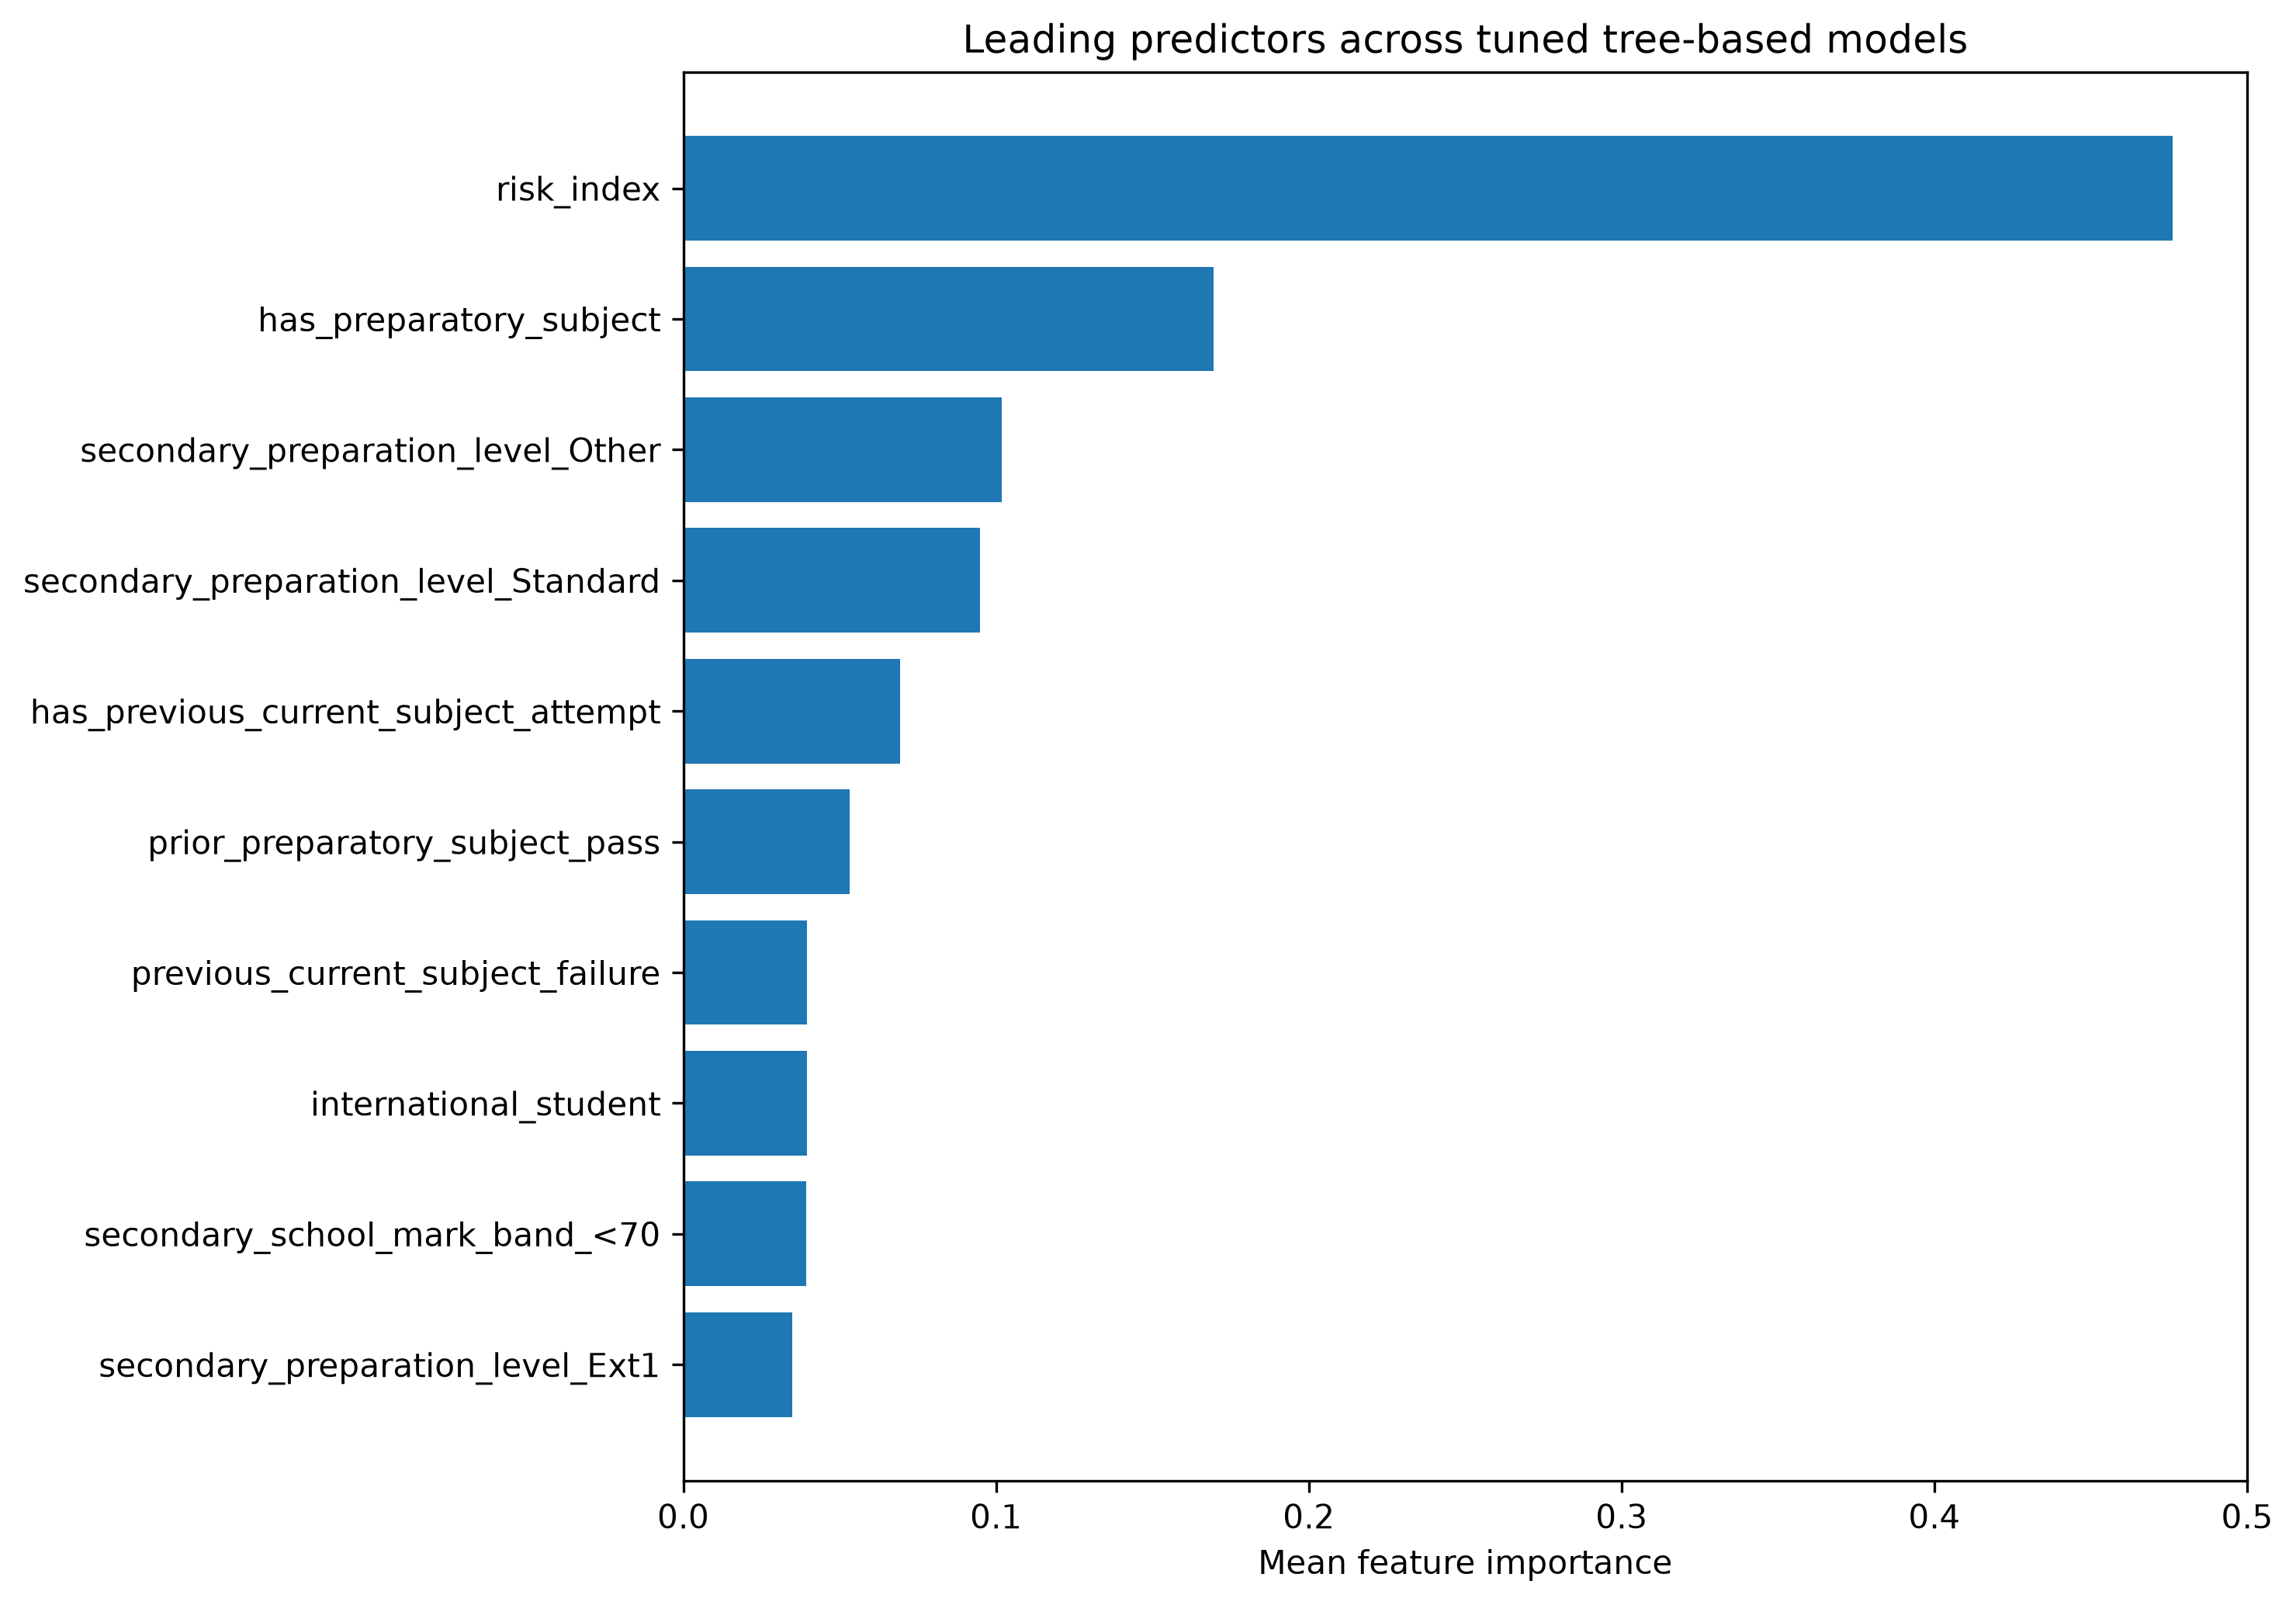
\includegraphics[
    width=\textwidth
]{../figures/fig_tuned_feature_importance_individual.png}
\caption{Individual feature importance values produced by the tuned tree-based models. Variables with larger importance contributed more strongly to the model's predictions.}
\label{fig:feature_importance_individual}
\end{figure}

Feature importance should be interpreted as a relative measure rather than an absolute effect size. The values indicate the comparative contribution of each predictor 
within a particular model and typically sum to one. Consequently, a feature with an importance of 0.30 contributed approximately twice as much to the model's predictive 
decisions as a feature with an importance of 0.15, but this does not imply a causal relationship.

In this study, feature importance was examined at two levels. Individual predictor variables were first evaluated within each model. Related variables were then 
aggregated into broader educational themes, including secondary mathematics preparation, previous university performance, preparatory mathematics, secondary school 
achievement, student characteristics, and the composite risk measure. This grouped interpretation provides a clearer educational perspective while preserving the 
underlying machine learning results.


\subsection{Grouped Feature Importance}

Individual feature importance values provide detailed information about the contribution of specific predictor variables. However, educational researchers are often 
interested in broader concepts rather than individual dummy-coded variables. For example, several variables may represent different levels of secondary mathematics 
preparation, while others describe previous university performance or participation in preparatory mathematics subjects.

To improve interpretability, this study grouped related predictor variables into educational themes before calculating their combined importance. This approach 
preserves the predictive information produced by the machine learning models while presenting the results in a form that is more closely aligned with educational theory 
and practice. Rather than interpreting numerous individual variables, readers can evaluate the relative importance of broader constructs that are meaningful within the 
context of student transition. The resulting grouped feature importance values are presented in Figure~\ref{fig:feature_importance_grouped}, providing an educational 
interpretation of the model outputs by aggregating related predictors into broader conceptual themes.

\begin{figure}[ht]
\centering
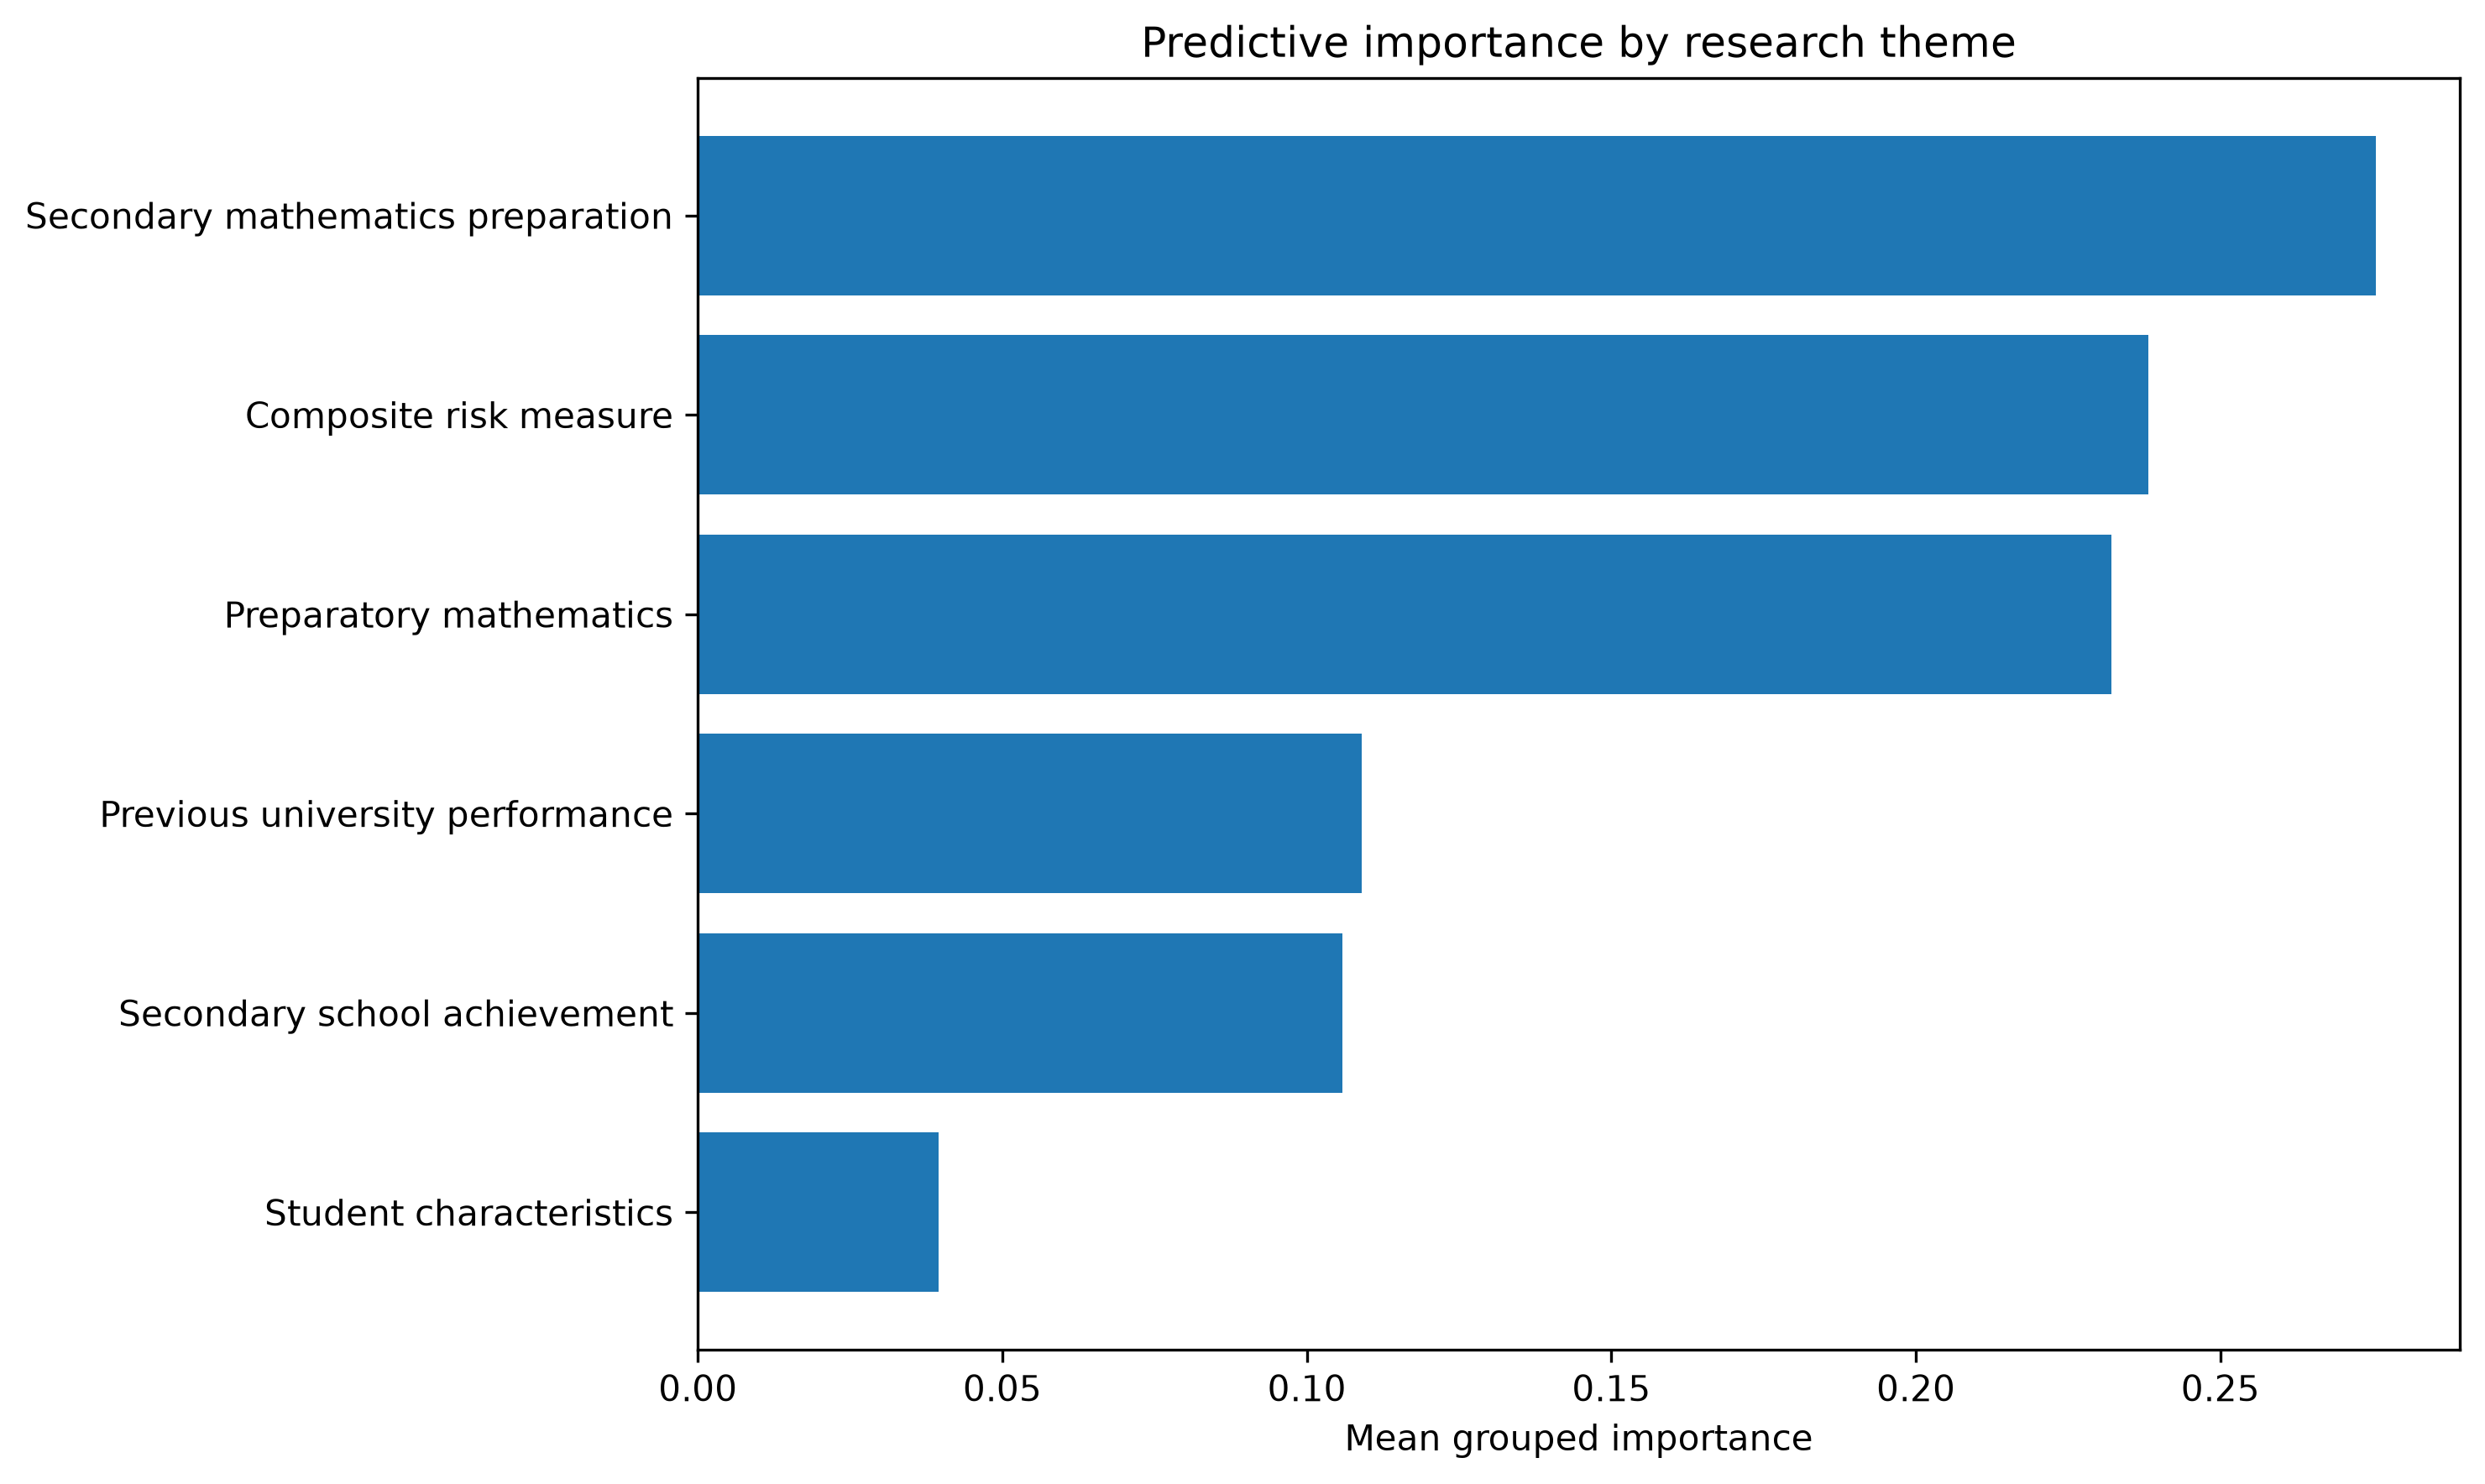
\includegraphics[
    width=\textwidth
]{../figures/fig_tuned_feature_importance_grouped.png}
\caption{Grouped feature importance values showing the relative contribution of broader educational themes across the tuned tree-based models.}
\label{fig:feature_importance_grouped}
\end{figure}

Grouping feature importance therefore provides an additional interpretative layer. It bridges the gap between machine learning outputs and educational understanding by 
translating technical model results into concepts that can be discussed within the broader literature on student preparation, transition, and academic success.

\subsection*{Part III — Model Development and Evaluation}
\subsection{Training and Test Data}

A fundamental principle of machine learning is that model performance should be evaluated using data that were not used during model training. If a model is assessed 
only on the observations from which it learned, the reported performance is likely to be overly optimistic because the model has already seen those examples.

To address this issue, the available data are commonly divided into two subsets. The training dataset is used to construct and tune the model, while the test dataset is 
reserved for an independent evaluation of predictive performance. The test data therefore provide a more realistic indication of how well the model is expected to perform 
when applied to new students.

This study adopted a reproducible train--test split, ensuring that all candidate models were evaluated using the same independent test dataset. This approach provides a 
fair comparison between models and reduces the likelihood that reported performance reflects random variation in the training data rather than genuine predictive capability.


\subsection{Cross-Validation}

A single train--test split provides one estimate of model performance, but the result may depend on the particular observations assigned to each subset. 
Cross-validation reduces this dependence by repeatedly dividing the training data into different partitions and evaluating the model across multiple iterations.

In (k)-fold cross-validation, the training data are divided into (k) approximately equal subsets. During each iteration, one subset is reserved for validation 
while the remaining subsets are used for model training. This process is repeated until every subset has served as the validation set exactly once. 
The resulting performance measures are then averaged to provide a more stable estimate of model performance.

Cross-validation is particularly valuable during model development because it helps identify models that generalise well rather than those that perform well 
only for a particular sample of training data. For this reason, it is commonly used during hyperparameter tuning before a final evaluation is performed on the 
independent test dataset.

\subsection{Hyperparameter Tuning}

Many machine learning models include settings, known as hyperparameters, that influence how the model is constructed. For example, a decision tree may be limited by its 
maximum depth, while a random forest requires the number of trees to be specified before training begins. These values are chosen by the researcher rather than learned 
directly from the data.

Hyperparameter tuning is the process of systematically evaluating different combinations of these settings to identify those that produce the best predictive performance. 
This evaluation is commonly performed using cross-validation so that each candidate configuration is assessed consistently across multiple training and validation partitions.

Careful hyperparameter tuning improves model robustness and reduces the risk of selecting a model that performs well only because of a particular choice of settings. 
In this study, all candidate models were tuned before their final performance was evaluated on the independent test dataset, ensuring that comparisons were both fair and 
reproducible.


\subsection{ROC Curves and Model Evaluation}

Receiver Operating Characteristic (ROC) curves provide a standard method for evaluating the discriminatory performance of binary classification models. Rather than 
assessing a model using a single classification threshold, an ROC curve summarises performance across all possible thresholds by plotting the true positive rate (sensitivity) 
against the false positive rate (1 -- specificity). This provides a threshold-independent assessment of how effectively a model distinguishes between the two outcome classes.

The overall discriminatory ability of a model is commonly summarised by the Area Under the ROC Curve (AUC). An AUC value of 0.5 indicates performance equivalent to random 
guessing, whereas a value of 1.0 represents perfect discrimination. In educational prediction studies, the ROC curve therefore provides a useful complement to measures such 
as accuracy, precision, and recall because it evaluates the model's ability to rank students according to their likelihood of success or failure, independent of any particular 
decision threshold. The ROC curves for the tuned decision tree and random forest models are presented in Figure~\ref{fig:roc_curve_primer}, allowing their discriminatory 
performance to be compared across all classification thresholds.

In this study, ROC curves were used to compare the predictive performance of the tuned decision tree and random forest models using the independent test dataset. This approach 
enabled the relative discriminatory performance of the competing models to be evaluated consistently and provided an objective basis for selecting the best-performing model 
while reducing the influence of any single classification threshold.

\begin{figure}[ht]
\centering
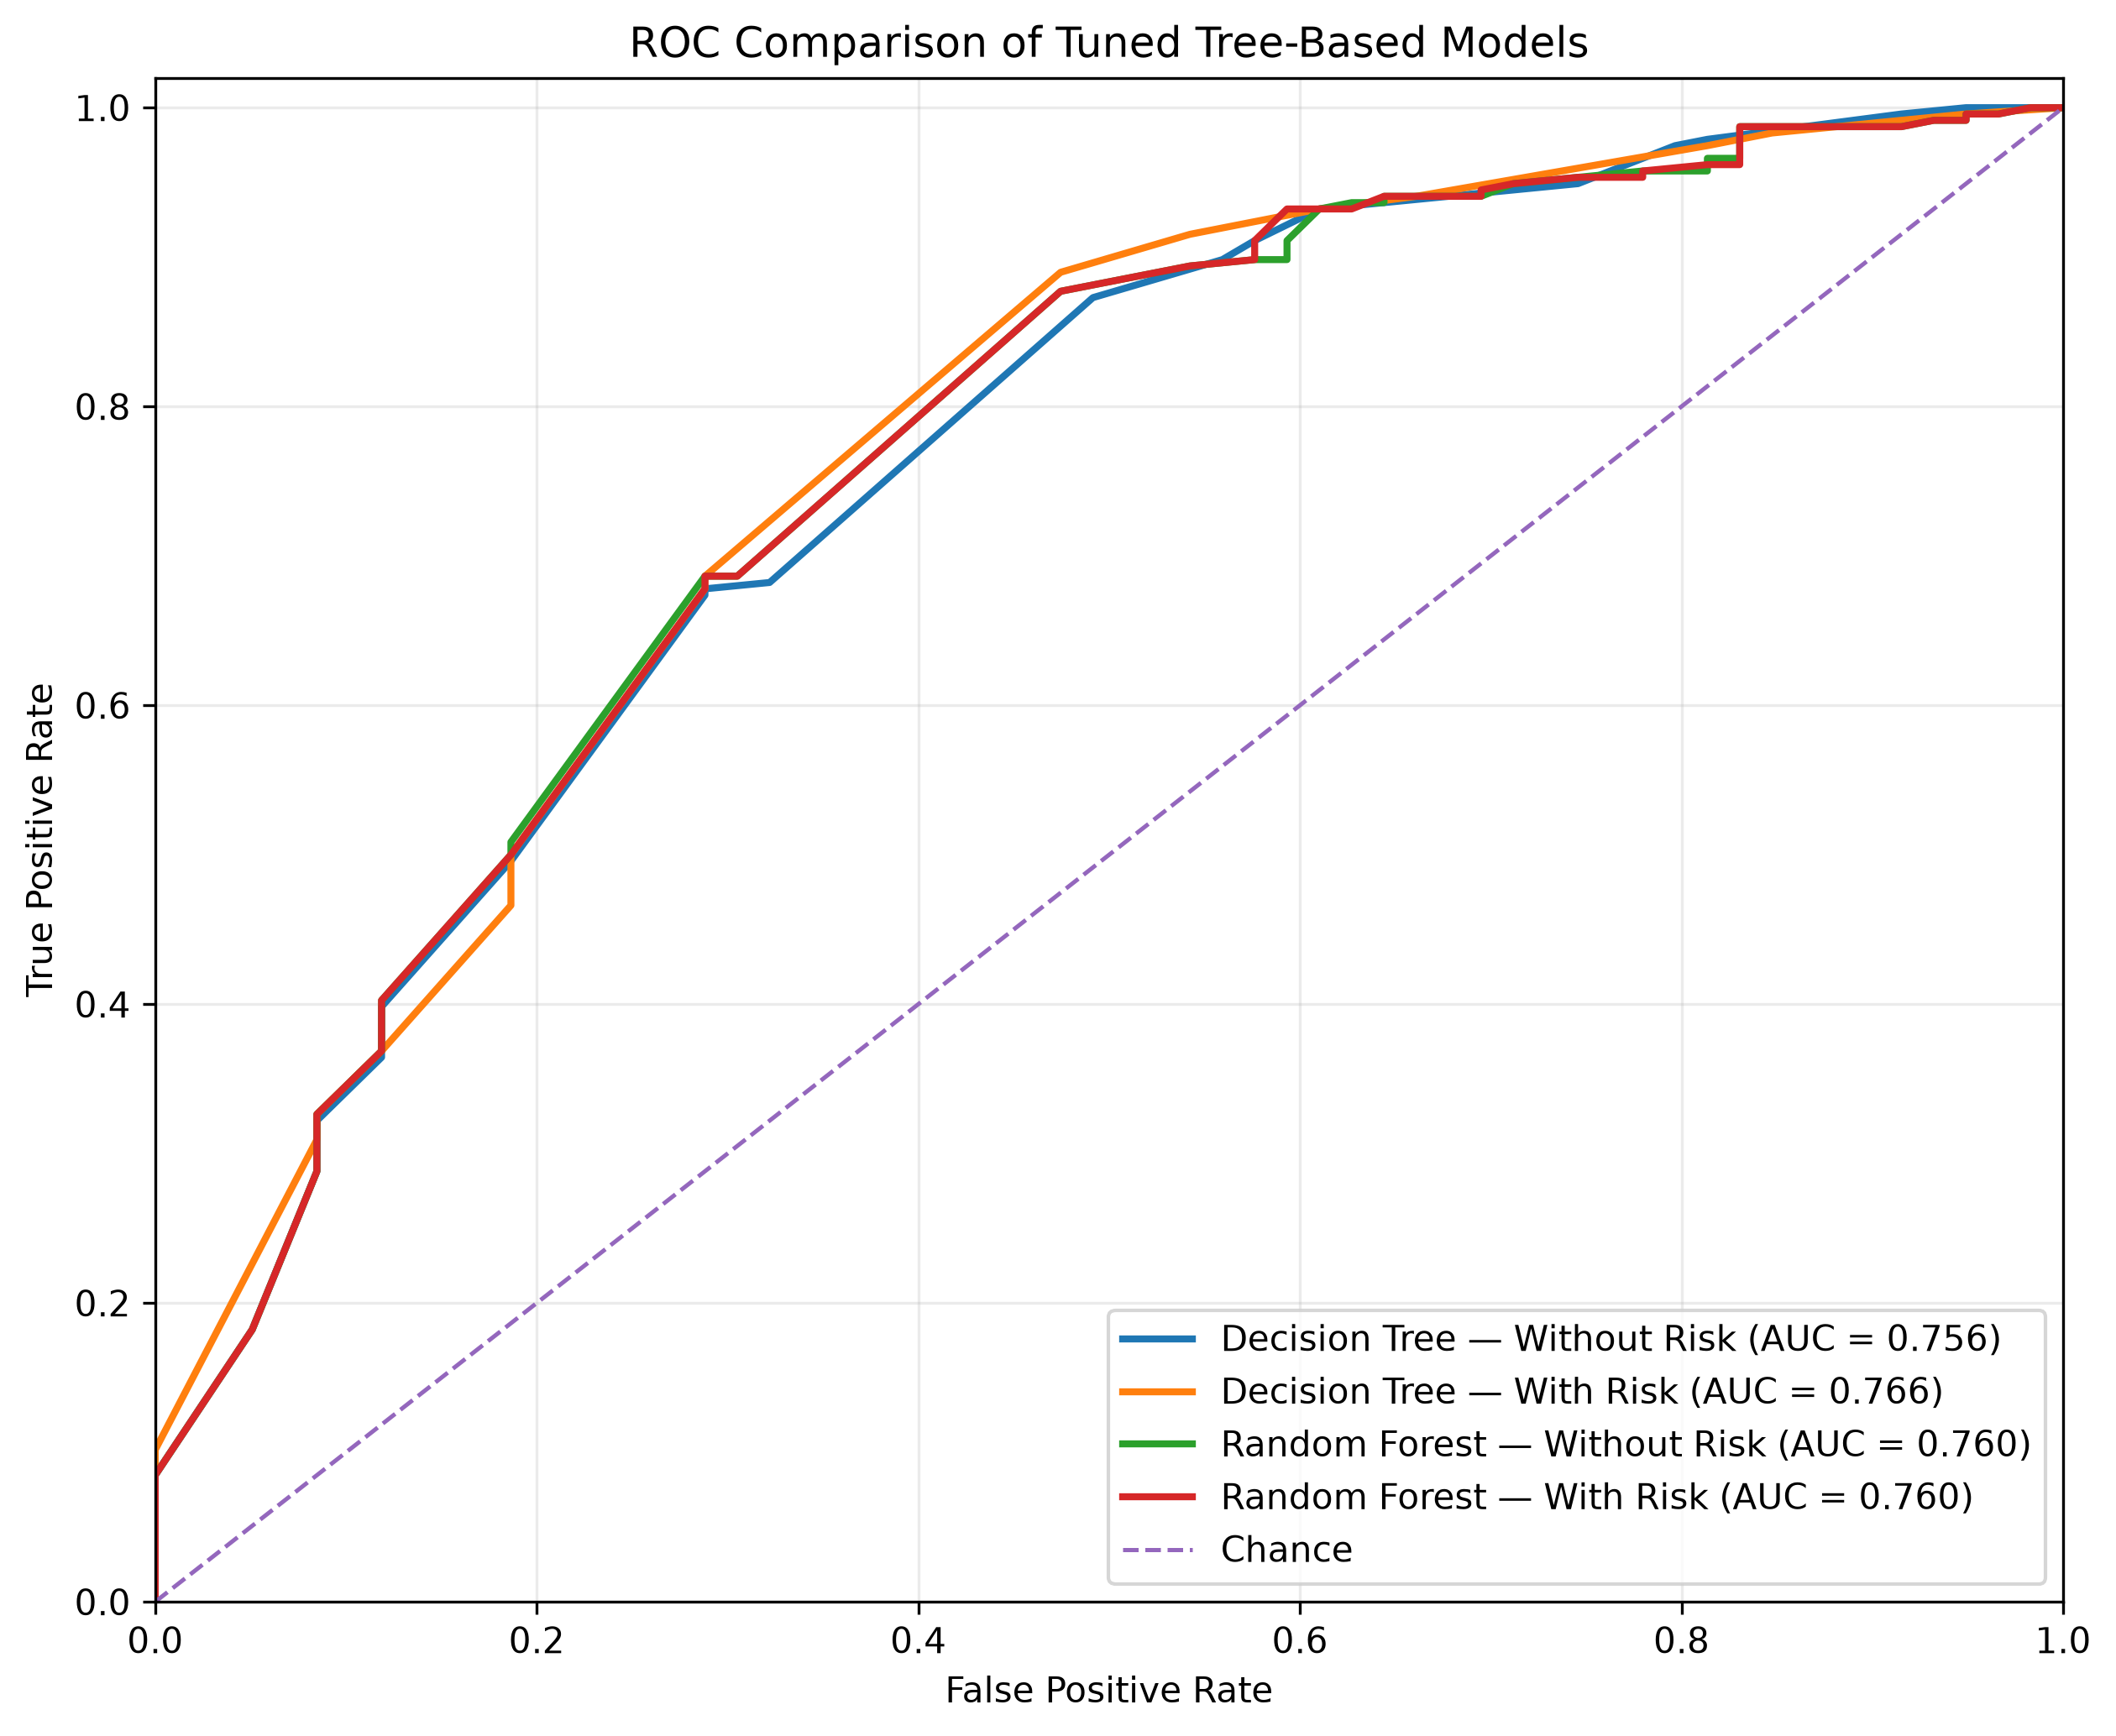
\includegraphics[width=0.75\textwidth]{../figures/fig_tuned_tree_roc_comparison.png}
\caption{Receiver Operating Characteristic (ROC) curves comparing the discrimination performance of the tuned tree-based models on the independent test dataset. Curves closer to the upper-left corner indicate stronger discriminatory performance, while the area under each curve (AUC) summarises overall model effectiveness across all classification thresholds.}
\label{fig:roc_curve_primer}
\end{figure}

\newpage

\subsection*{Part IV — Research Methodology}
\subsection{Why Statistical Models and Machine Learning Were Both Used}

Statistical modelling and machine learning provide complementary perspectives rather than competing methodologies. Statistical models are particularly valuable when the 
objective is to estimate relationships between variables, test hypotheses, and quantify uncertainty. Machine learning methods are designed to maximise predictive 
performance and to identify complex patterns that may not be apparent using traditional statistical techniques alone.

This study deliberately combined both approaches. Logistic regression provided a well-established statistical benchmark against which the machine learning models could be 
compared. Decision trees and random forests were then used to investigate predictive performance and to examine the relative importance of educational factors influencing 
student success.

Using both approaches strengthened the overall analysis. Agreement between the statistical and machine learning results increased confidence in the findings, 
while differences between the models provided additional insight into the strengths and limitations of each analytical approach.



\subsection{Reproducible Computational Workflows}

Reproducibility is a fundamental principle of modern computational research. A reproducible workflow ensures that the complete analysis, from data preparation to the 
final manuscript, can be repeated using the same source data and documented procedures. This reduces the likelihood of transcription errors, improves transparency, and 
enables other researchers to verify and extend the reported findings.

In this study, reproducibility was supported through an integrated computational workflow. Data preparation, statistical modelling, machine learning analyses, independent 
verification, figure generation, table production, and manuscript components were all produced automatically from the underlying analysis. The paper itself incorporated 
generated values directly from the analysis pipeline, ensuring consistency between reported results and computational outputs. The overall computational workflow 
developed for this research is summarised in Figure~\ref{fig:workflow_primer}, illustrating how the study progresses from raw research data through automated analysis, 
independent verification, and manuscript generation.

Such workflows provide benefits beyond a single study. They simplify maintenance, facilitate future analyses on new datasets, and support transparent, evidence-based 
educational research by ensuring that published results remain directly traceable to the underlying computations.

\begin{figure}[ht]
\centering
% TODO: Replace with workflow diagram
\fbox{\parbox{0.9\textwidth}{\centering
Figure A.6 Placeholder\\[1ex]
Reproducible Computational Workflow\\[2ex]

Raw Research Data\\
$\downarrow$\\
Data Preparation\\
$\downarrow$\\
Statistical Analysis\\
$\downarrow$\\
Machine Learning \hspace{2cm} Independent R Verification\\
\hspace{2.8cm}$\backslash$ \hspace{0.2cm}/\\
\hspace{2.9cm}$\downarrow$\\
Tables • Figures • Generated LaTeX Values\\
$\downarrow$\\
Automated Paper Generation\\
$\downarrow$\\
Publication-ready PDF}}
\caption{Overview of the reproducible computational workflow developed for this study, illustrating the progression from raw research data through analysis, independent verification, automated reporting, and final manuscript generation.}
\label{fig:workflow_primer}
\end{figure}

\newpage
\bibliographystyle{apalike}
\bibliography{bib/references}
\newpage

\appendix

\section{GitHub repository}

This report was generated semi-automatically, using a Transition Analysis Toolkit. The toolkit resides as a repo on GitHub, and can be cloned and tested for research purposes.

The design of the toolkit allows specific variables to be imbedded in LaTex dynamically. So as experiment values change, they are automatically updated in the LaTex documents, 
including tables and figures.

The narrative and subsequent observations can then be updated manually as needed.

Shell commands activate various parts of the package from incremental tests to a complete LaTex report. The intention was to generate a journal paper ready to serve from a single workflow environment.



\medskip

\noindent
Repository: \\

\bigskip

\href{https://github.com/jasonnstanley/transition_analysis}{\nolinkurl{https://github.com/jasonnstanley/transition_analysis}}


\section{Machine Learning Primer}

This study is accompanied by a standalone machine learning primer that will change and evolve as it is updated and introduces the statistical and machine learning concepts used throughout the analysis, including decision trees, random forests, receiver operating characteristic (ROC) curves, feature importance, and the reproducible computational workflow.

The primer is maintained separately from this paper so that it can evolve as an independent educational resource and be reused across future research and teaching projects.


\medskip

\noindent
Repository: \\

\bigskip

\href{https://github.com/jasonnstanley/transition_analysis_ml_primer}{\nolinkurl{https://github.com/jasonnstanley/transition_analysis_ml_primer}}

\end{document}